\documentclass[a4paper,11pt]{article}
\usepackage[top=2.5cm,bottom=3cm,right=3cm,left=3cm]{geometry}
\usepackage[utf8]{inputenc}
\usepackage[T1]{fontenc}
\usepackage[french]{babel}
\usepackage{graphicx,graphics,textcomp,setspace,lettrine}
\usepackage{amsmath,amssymb,amsfonts,indentfirst}
\usepackage[toc,page]{appendix} 
\usepackage{float}
\usepackage{array}
\usepackage{comment}
\usepackage{xcolor}
\usepackage{listings}
\usepackage{blindtext}
\usepackage{titling}
\usepackage{multicol}

\usepackage[english, status=draft]{fixme}
\fxusetheme{color}

\lstset{numbers=left,
numberstyle=\tiny \bf ,
stepnumber=1,
numbersep=10pt,
firstnumber=1,
numberfirstline=true}

\lstset{frame=TBlr,
rulesepcolor=\color{black}}

\DeclareMathOperator{\e}{e}

\usepackage{fancyhdr}
\pagestyle{fancy}

\renewcommand{\headrulewidth}{1pt}
\fancyhead[L]{\leftmark}
\fancyhead[R]{}

\renewcommand{\footrulewidth}{1pt}
\fancyfoot[C]{\textbf{\thepage}} 
\fancyfoot[L]{}

\graphicspath{{results/}}

\title{{\textsc{\Large{Rapport de Méthodologie}\\ [3cm]
      \textbf{\LARGE{Amas de galaxies \\ de Planck}} \\ [0.6cm] 
Etude à travers l'effet \\ Sunyaev-Zel’dovich}} \\[2cm]}
\vfill
\author{Geoffroy de la Vieuville \\ Antoine Marchal}
\date{}


\begin{document}
\begin{titlingpage}
\maketitle
\begin{abstract}
  La collaboration Planck a extrait sur l'ensemble de la mission un
  catalogue d'amas de galaxie (PSZ2) basé sur la détection de l'effect
  Sunyaev-Zel’dovich (SZ). Nous avons, à l'aide de celui-ci,
  reconstruit par ILC (Internal Linear Combination) des estimateurs du
  CMB et de l'effet SZ thermique pour chaque amas. 
  L'étude des poids $w(\nu)$ donnés aux six fréquences des 
  maps de Planck nous apportent une vision sur les différents
  phénomènes physique pouvant intervenir dans l'extraction de ces données. Enfin,
  l'application d'une photométrie d'ouverture nous a ensuite permis 
  d'étudier quelques propriétés de ces amas comme le flux $F=f(z)$ 
  ou encore le rayon critique photométrique $R_{60}=f(z)$.
\end{abstract}
\end{titlingpage}
%\tableofcontents
%\thispagestyle{empty}
\newpage
\section{L'effet Sunyaev-Zel’dovich}

\begin{figure}[b!]
  \centering
  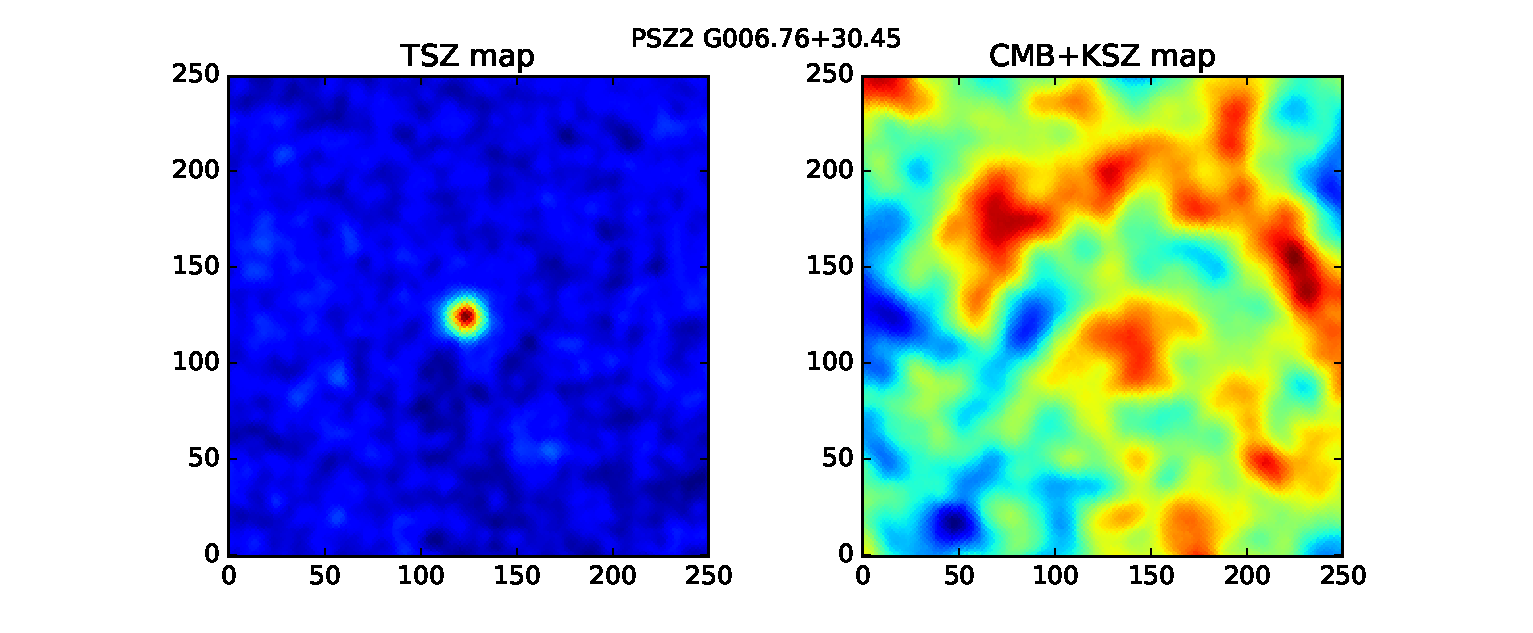
\includegraphics[width=4.5in]{sz_effect.eps}
  \label{sz_effect}
  \caption{Séparation par méthode ILC de la composante TSZ (gauche) et de la
    composante CMB+KSZ (droite) pour l'amas G006.76+30.45 du catalogue
  PSZ2}
\end{figure}

L'effet Sunyaev-Zel’dovich \cite{Sunyaev} est provoqué par la diffusion Compton
Inverse des photons du CMB par le gaz d'électrons chaud ($k_B T_e
\lesssim 15$ KeV) présent dans les amas de galaxies. Son application à
la cosmologie est capitale puisqu'il est de part sa nature
théoriquement indépendant du redshift. Il permet donc l'étude de la
distribution des amas qui est un enjeux important dans la
compréhension du modèle standard de la cosmologie et notamment de la
formation des grandes structures. Son équation est donnée par : 

\begin{align*}
  \frac{\Delta T_{SZE}}{T_{CMB}} = f(\nu) \times  y
\end{align*}

\begin{multicols}{2}\noindent
\begin{align*}
  y = \int_{l.o.s} \frac{kT_e}{m_e c^2} n_e \sigma_T dl 
\end{align*}
\begin{align*}
  f(\nu) = \frac{h \nu}{k T_{CMB}} \frac{\e^{x(\nu) + 1}}{\e^{x(\nu)
  -1}} - 4
\end{align*}
\end{multicols}

où $k$ is est la constante Boltzmann, $m_e$ la masse des electrons, $c$
la vitesse de la lumière, $\sigma_T$ la section efficace de Thomson, 
$n_e$ la densité d'electrons et $T_e$ la température des electrons.

Deux composantes sont à distinguer, l'effet SZ thermique (TSZ) et
l'effet SZ cinétique (KSZ). La deuxième composante est simplement dù à un effet
Doppler additionnel. 

\section{Application de la méthode ILC}

\begin{figure}[b!]
  \centering
  \label{w_lat}
  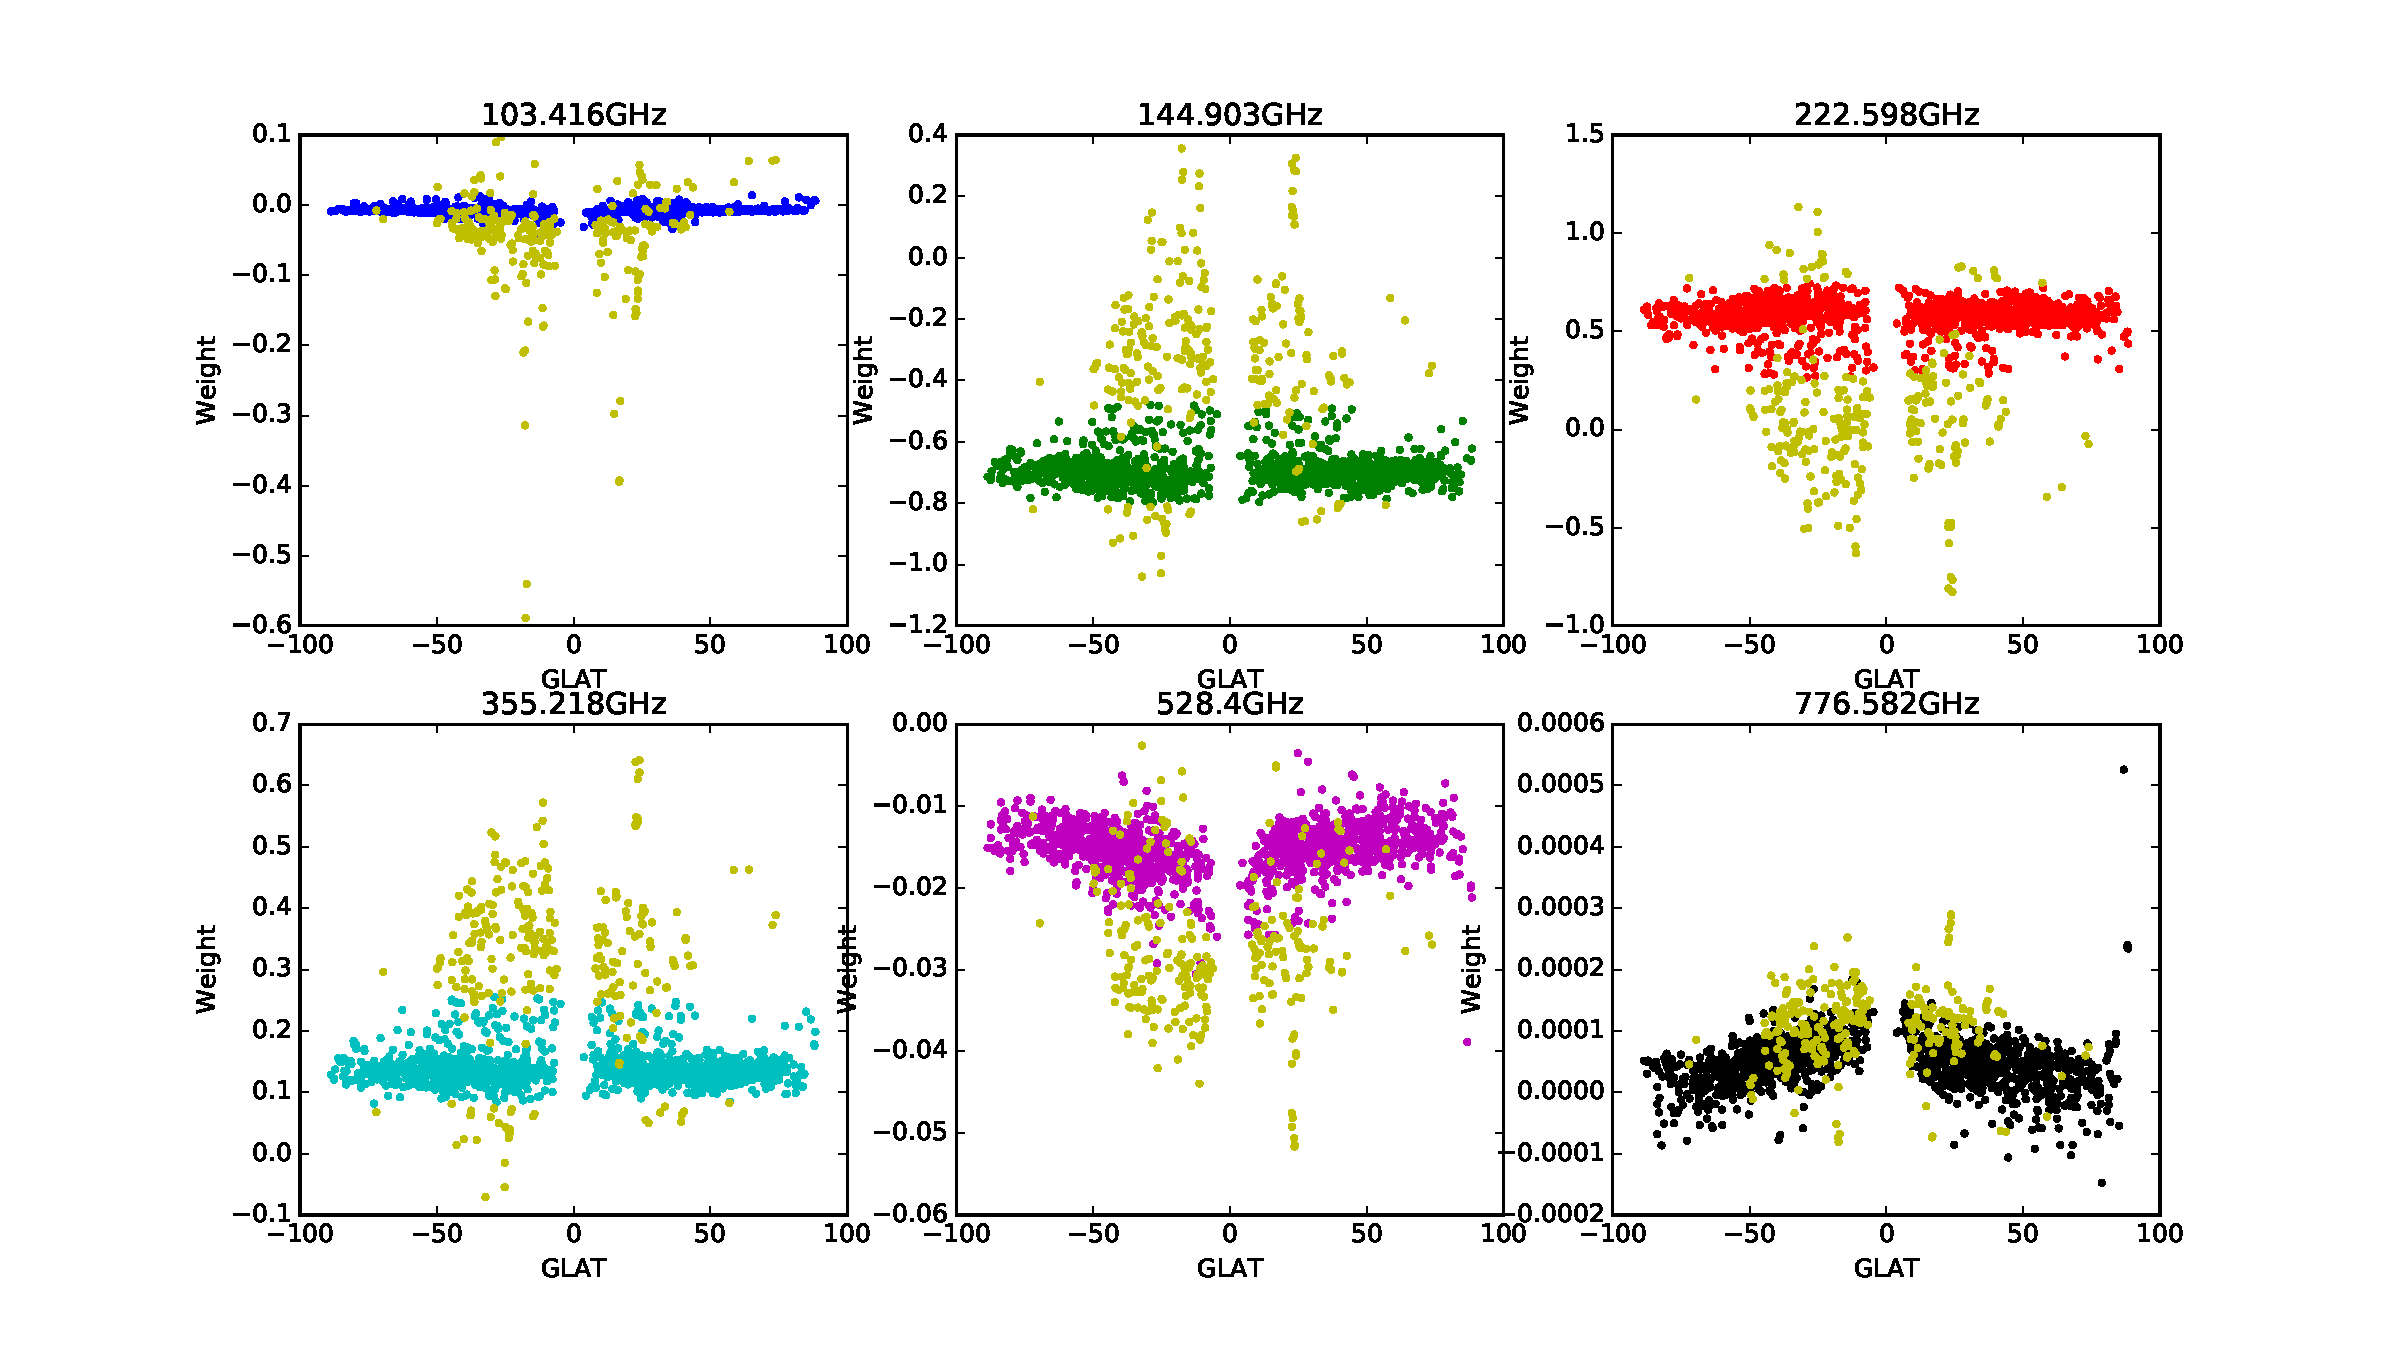
\includegraphics[width=6in]{w_lat.pdf}
  \caption{Etude des poids appliqués à chacune des six fréquences en
    fonction de la latitude en coordonnée galactique pour
  l'ensemble de 1653 amas du catalogue. En jaune sont représenté les
  amas exclus qui s'écarte de plus d'un $\sigma$ de la valeur moyenne.}
\end{figure}

L'ILC utilisé ici est basé sur l'article de Remazeilles M. \&
al. \cite{Remazeilles}. Cette méthode nous permet d'obtenir  une
estimation indépendante du CMB et de l'effet SZ. L'estimateur
permettant la variance minimum est donné par la combinaison linéaire: 

\begin{align*}
  \widehat{\textbf{s}} = \textbf{w}^t \textbf{x}
\end{align*}

\begin{align}
  \label{eq::w}
  \textbf{w}^t = \frac{\left( \textbf{b}^t\widehat{R}^{-1} \textbf{b}
    \right) \textbf{a}^t \widehat{R}^{-1} - \left( \textbf{a}^t\widehat{R}^{-1} \textbf{b}
    \right) \textbf{b}^t \widehat{R}^{-1}}{\left( \textbf{a}^t\widehat{R}^{-1} \textbf{a}
    \right) \left( \textbf{b}^t\widehat{R}^{-1} \textbf{b}
    \right) - \left( \textbf{a}^t\widehat{R}^{-1} \textbf{b}
    \right)^2}
\end{align}

où $\widehat{R}$ est la matrice de covariance empirique des cartes
observationnelles, $a = (1, 1, ..., 1)^t$ et b est le vecteur de
l'effet SZ thermique donné par $f(\nu)$. A partir des coordonnées
galactiques des amas de PSZ2 nous appliquons une ILC sur chaque amas
contenu dans un patch de dimensions FIXME \fxwarning{dimension physique
  patch} extrait au préalable de la sphère celeste de Planck par
projection tangentielle. 
Un des résultats de l'ILC est représenté Figure \ref{sz_effect}. La
map en température de l'effet SZ thermique est représentée sur lea
partie gauche et le CMB sur la partie droite. Il est intéressant de
constater qu'actuellement l'effet SZ cinétique est indiscernable du
CMB par cette méthode.  
Ce qui va nous interesser par la suite est l'étude du comportement des
poids appliqués à chaque fréquence. En effet le calcul présenté
équation \eqref{eq::w} est fonction de la matrice de corélation $R$ entre
les six cartes de fréquences. Cependant, $R$ peut être plus ou moins affecté par
différents effets (citués à des fréquences voisines de celles de l'effet SZ et
du CMB) présent en avant plan : le rayonnement synchrotron et le
rayonnement de freinage, la galaxie et les poussières, ou encore le bruit du
détecteur.  \\

La Figure \ref{w_lat} nous montre, pour chaque fréquence, le poids
des amas du catalogue en fontion de la latitude donnée en coordonnées
galactiques. On distingue bien une corélation entre ces deux
variables. Ce sont dans les deux fréqences les plus haute que le
perturbation est la plus grande (ie. la galaxie y est le plus
présente). Pour continuer notre analyse et effectuer de la photométrie
d'ouverture sur les amas, nous avons décider d'exclure les amas dont
le poids s'écarte de plus d'un $\sigma$ de la valeur moyenne, où
$\sigma$ représente la déviation standard sur l'ensemble 1653 amas. \\

Nous pouvons voir sur la Figure \ref{w_full} les poids moyenné sur
l'ensemble des amas du catalogue (bleu ciel) et sur l'ensemble des
amas selectionné (bleu foncé) en fonction de la fréquence. De plus
nous représentons les mêmes grandeurs calculer pour chacune des maps
complète de Planck. On observe un bon accord pour les 4 fréquences les
plus hautes et un désaccord pour les deux les plus basses. A basse
fréquence l'émission synchrotron de la galaxie peut en effet induire
ce décalage. Il n'est pas présent sur les amas du catalogue car
beaucoup moins nombreux dans le plan de la galaxie du simplement à un
effet observationel. 

\begin{figure}[h!]
  \centering
  \label{w_full}
  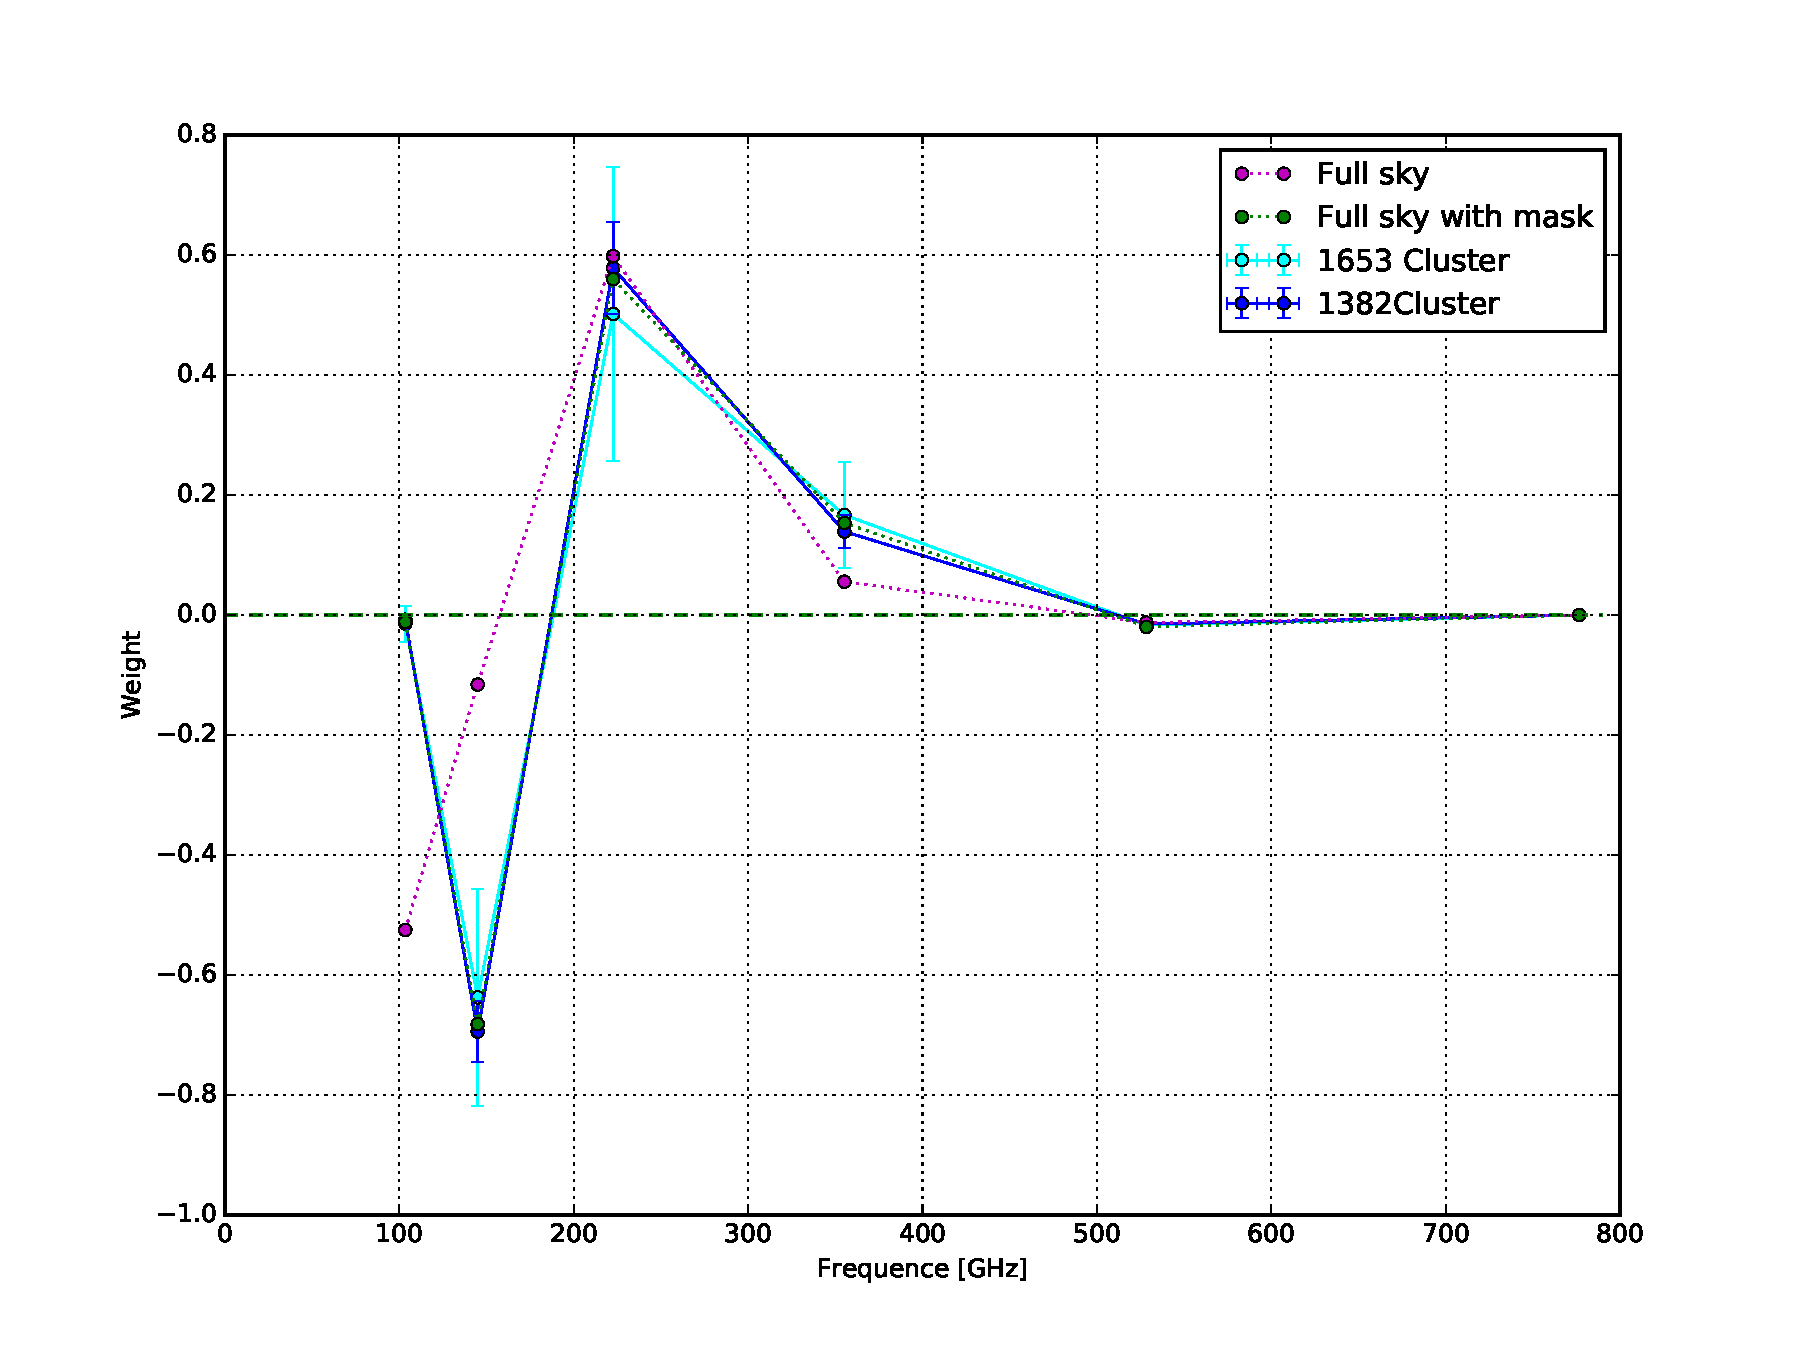
\includegraphics[width=4.6in]{w_full.pdf}
  \caption{Poids moyen de l'ensemble des amas du catalogue (bleu ciel) et sur
    l'ensemble des amas selectionnés (bleu foncé) en fonction
    de la fréquence. En violet sont réprésenté ces grandeurs pour
    l'ensemble des maps Planck.}
\end{figure}
  

\section{Photémétrie d'ouverture}
\section{Résultats et discussion}

\begin{figure}[h!]
  \centering
  \label{rslt_1}
  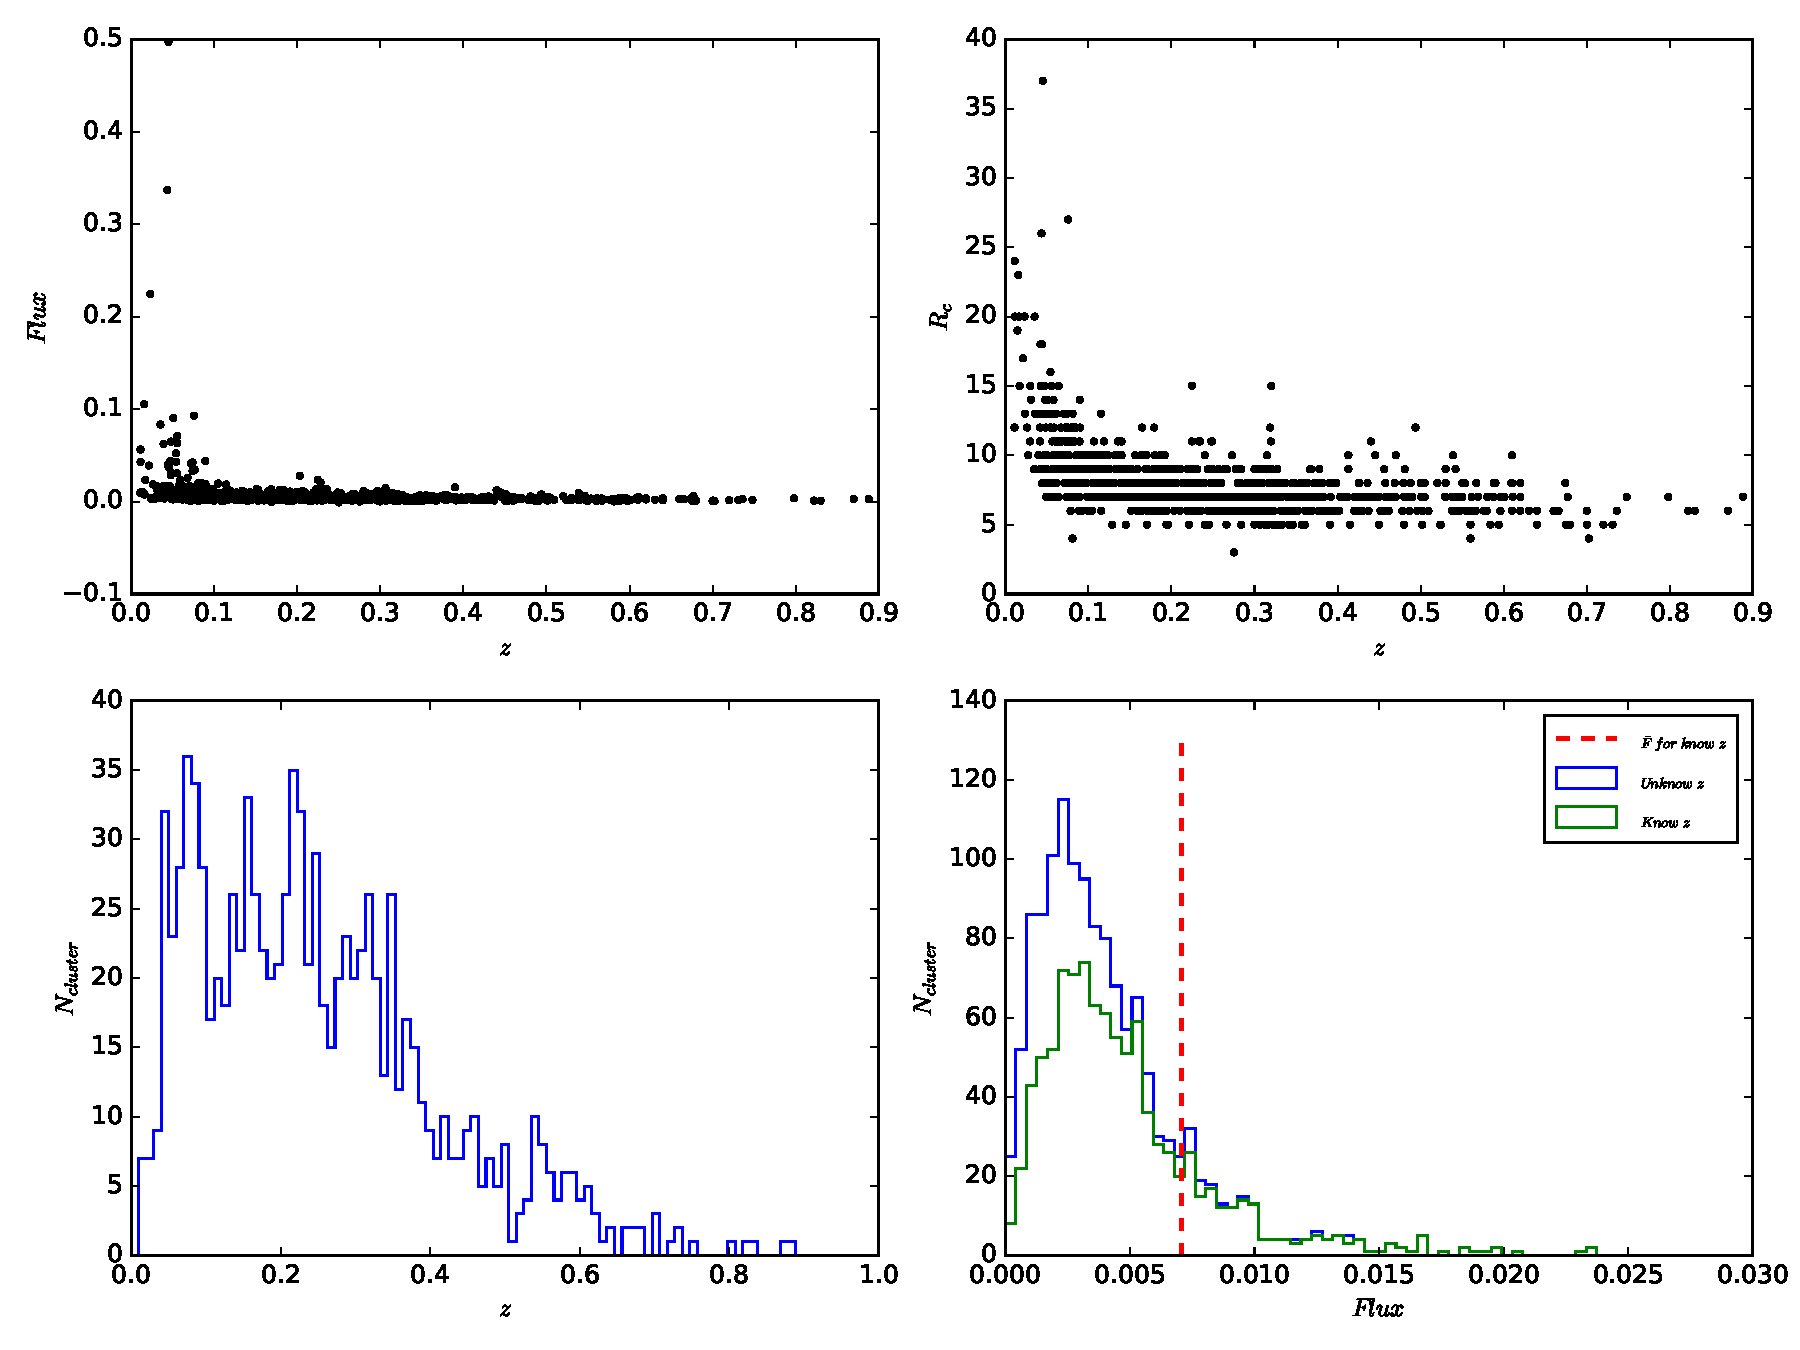
\includegraphics[width=4in]{rslt_1.pdf}
  \caption{}
\end{figure}


\newpage
\begin{thebibliography}{2}
  \addcontentsline{toc}{chapter}{Bibliographie} 

\bibitem{Sunyaev} Sunyaev, R. A., \& Zeldovich, Y. B. 1972, Comments on
  Astrophysics and Space Physics, 4, 173 \\
  
\bibitem{Remazeilles}Remazeilles M. \& al., CMB and SZ effect
  separation with Constrained Internal Linear Combinations, 
  Mon. Not. R. Astron. Soc. 410, 2481–2487 (2011)  \\
  
\end{thebibliography}
\listoffixmes
\end{document}

